
\documentclass[
  bibliography=totoc,     % Literatur im Inhaltsverzeichnis
  captions=tableheading,  % Tabellenüberschriften
  titlepage=firstiscover, % Titelseite ist Deckblatt
  ngerman,
  a4paper
]{article}


\usepackage{lmodern}%Font
\usepackage[T1]{fontenc}
\usepackage[utf8]{inputenc}
\usepackage{scrhack}% Paket float verbessern
\usepackage{longtable}
\usepackage{multicol}% columns
%\usepackage[top=1cm,left=0.8cm,bottom=1.5cm,right=0.8cm]{geometry}

\usepackage[parfill]{parskip}%linebreaks instead of indention after paragraphs

\usepackage[aux]{rerunfilecheck}% Warnung, falls nochmal kompiliert werden muss
\usepackage{fixltx2e} % provides \textsubscript

\usepackage[shorthands=off,ngerman]{babel}% deutsche Spracheinstellungen

\usepackage{amsmath}% viele Mathe-Symbole
\usepackage{amssymb}
\usepackage{mathtools}
\usepackage{dsfont}
\usepackage{nicefrac}

\usepackage{adjustbox}

\usepackage{blindtext}
\usepackage{titlesec}%Page breaks before new sections
\newcommand{\sectionbreak}{\clearpage}

% traditionelle Fonts für Mathematik
%\setmathfont{Latin Modern Math}
%\setmathfont{XITS Math}[range={scr, bfscr}]
%\setmathfont{XITS Math}[range={cal, bfcal}, StylisticSet=1]

% Zahlen und Einheiten
\usepackage[
  locale=DE,                 % deutsche Einstellungen
  separate-uncertainty=true, % immer Fehler mit \pm
  per-mode=reciprocal,       % ^-1 für inverse Einheiten
  output-decimal-marker=.,   % . statt , für Dezimalzahlen
]{siunitx}




% chemische Formeln
\usepackage[
  version=4,
  math-greek=default, % ┐ mit unicode-math zusammenarbeiten
  text-greek=default, % ┘
]{mhchem}

\usepackage[autostyle]{csquotes}% richtige Anführungszeichen
\usepackage{upquote}%straight quotes in verbatim environments
\usepackage{xfrac}% schöne Brüche im Text
\usepackage{grffile}% größere Variation von Dateinamen möglich
\usepackage{booktabs}% schöne Tabellen
\usepackage{microtype}% Verbesserungen am Schriftbild
\setlength{\emergencystretch}{3em}  % prevent overfull lines

% Standardplatzierung für Floats einstellen
\usepackage{float}
\floatplacement{figure}{htbp}
\floatplacement{table}{htbp}
\usepackage[% Floats innerhalb einer Section halten
  section, % Floats innerhalb der Section halten
  below,   % unterhalb der Section aber auf der selben Seite ist ok
]{placeins}

\usepackage{pdflscape}% Seite drehen für breite Tabellen

% Captions schöner machen.
\usepackage[
  labelfont=bf,        % Tabelle x: Abbildung y: ist jetzt fett
  font=small,          % Schrift etwas kleiner als Dokument
  width=0.9\textwidth, % maximale Breite einer Caption schmaler
]{caption}
% subfigure, subtable, subref
\usepackage{subcaption}

\usepackage{graphicx}% Grafiken können eingebunden werden

% Hyperlinks im Dokument
\usepackage[
  unicode,        % Unicode in PDF-Attributen erlauben
  pdfusetitle,    % Titel, Autoren und Datum als PDF-Attribute
  pdfcreator={},  % ┐ PDF-Attribute säubern
  pdfproducer={}, % ┘
]{hyperref}
\hypersetup{breaklinks=true,
            bookmarks=true,
            colorlinks=true,
            citecolor=blue,
            urlcolor=blue,
            linkcolor=magenta,
            pdfborder={0 0 0}
            }
\urlstyle{same}  % don't use monospace font for urls

% Literaturverzeichnis
\usepackage[
  backend=biber,
]{biblatex}
% Quellendatenbank
\addbibresource{lit.bib}
\addbibresource{programme.bib}


% erweiterte Bookmarks im PDF
\usepackage{bookmark}

% Trennung von Wörtern mit Strichen
\usepackage[shortcuts]{extdash}

% --- Macro \xvec
\makeatletter
\newlength\xvec@height%
\newlength\xvec@depth%
\newlength\xvec@width%
\newcommand{\xvec}[2][]{%
  \ifmmode%
    \settoheight{\xvec@height}{$#2$}%
    \settodepth{\xvec@depth}{$#2$}%
    \settowidth{\xvec@width}{$#2$}%
  \else%
    \settoheight{\xvec@height}{#2}%
    \settodepth{\xvec@depth}{#2}%
    \settowidth{\xvec@width}{#2}%
  \fi%
  \def\xvec@arg{#1}%
  \def\xvec@dd{:}%
  \def\xvec@d{.}%
  \raisebox{.2ex}{\raisebox{\xvec@height}{\rlap{%
    \kern.05em%  (Because left edge of drawing is at .05em)
    \begin{tikzpicture}[scale=1]
    \pgfsetroundcap
    \draw (.05em,0)--(\xvec@width-.05em,0);
    \draw (\xvec@width-.05em,0)--(\xvec@width-.15em, .075em);
    \draw (\xvec@width-.05em,0)--(\xvec@width-.15em,-.075em);
    \ifx\xvec@arg\xvec@d%
      \fill(\xvec@width*.45,.5ex) circle (.5pt);%
    \else\ifx\xvec@arg\xvec@dd%
      \fill(\xvec@width*.30,.5ex) circle (.5pt);%
      \fill(\xvec@width*.65,.5ex) circle (.5pt);%
    \fi\fi%
    \end{tikzpicture}%
  }}}%
  #2%
}
\makeatother


%make parantheses scale in math mode
\makeatletter
\def\resetMathstrut@{%
  \setbox\z@\hbox{%
    \mathchardef\@tempa\mathcode`\[\relax
    \def\@tempb##1"##2##3{\the\textfont"##3\char"}%
    \expandafter\@tempb\meaning\@tempa \relax
  }%
  \ht\Mathstrutbox@\ht\z@ \dp\Mathstrutbox@\dp\z@}
\makeatother
\begingroup
  \catcode`(\active \xdef({\left\string(}
  \catcode`)\active \xdef){\right\string)}
\endgroup
\mathcode`(="8000 \mathcode`)="8000

%increase math spacing between lines with fractions
\makeatletter

\newlength\minalignvsep
\def\align@preamble{%
   &\hfil
    \setboxz@h{\@lign$\m@th\displaystyle{##}$}%
    \ifnum\row@>\@ne
    \ifdim\ht\z@>\ht\strutbox@
    \dimen@\ht\z@
    \advance\dimen@\minalignvsep
    \ht\strutbox\dimen@
    \fi\fi
    \strut@
    \ifmeasuring@\savefieldlength@\fi
    \set@field
    \tabskip\z@skip
   &\setboxz@h{\@lign$\m@th\displaystyle{{}##}$}%
    \ifnum\row@>\@ne
    \ifdim\ht\z@>\ht\strutbox@
    \dimen@\ht\z@
    \advance\dimen@\minalignvsep
    \ht\strutbox@\dimen@
    \fi\fi
    \strut@
    \ifmeasuring@\savefieldlength@\fi
    \set@field
    \hfil
    \tabskip\alignsep@
}
\makeatother

\minalignvsep.15em


%align-nummerierung berichtigen
%\numberwithin{equation}{subsection}
%\renewcommand{\theequation}{\thesubsection.\arabic{equation}}

\DeclareMathOperator{\const}{const.}

\author{
  Thea Schneider%
  \texorpdfstring{
    \\
    \href{mailto:thea.schneider@udo.edu}{thea.schneider@udo.edu}
  }{}%
  \texorpdfstring{\and}{, }
  Max Pernklau%
  \texorpdfstring{
    \\
    \href{mailto:max.pernklau@udo.edu}{max.pernklau@udo.edu}
  }{}%
}
%\publishers{TU Dortmund – Fakultät Physik}

\newcommand{\integral}[4]{\int\displaylimits_{#3}^{#4} #1 \, \mathrm{d} #2}
\makeatletter
\newcommand\primitiveinput[1]
{\@@input #1 }
\makeatother

\newcommand*\diff{\mathop{}\!\mathrm{d}}
\newcommand*\Diff[1]{\mathop{}\!\mathrm{d^#1}}
\newcommand{\partialfrac}[2]{\frac{\mathrm{\partial}#1}{\mathrm{\partial}#2}}

\newcommand*\inv[1]{#1^{-1}}

\newcommand*{\estimates}{\stackrel{\scriptscriptstyle\wedge}{=}}

\DeclareSIUnit[number-unit-product = \,]{\permil}{\text{\textperthousand}}

\newcommand{\HRule}{\rule{\linewidth}{0.5mm}}

\begin{document}
\begin{titlepage}
\begin{center}

~\\[1cm]


\textsc{\Large Praktikumsprotokoll des 24.5.2016}\\

% Title
\huge{ \bfseries Messung der Suszeptibilität paramagnetischer Substanzen}\\[1em]


% Author and supervisor
\begin{minipage}{0.4\textwidth}
\begin{flushleft} \large
Thea \textsc{Schneider}\\
thea.schneider@udo.edu
\end{flushleft}
\end{minipage}
\begin{minipage}{0.4\textwidth}
\begin{flushright} \large
Max \textsc{Pernklau}\\
max.pernklau@udo.edu
\end{flushright}
\end{minipage}
%\textsc{\large \newline Durchführung: 15.12.2015} \\

\vfill

{\large \today}

\end{center}
\end{titlepage}


\thispagestyle{empty}
%\tableofcontents
%\newpage

%\begin{multicols}{2}
\section{Abstract}
\label{sec:Abstract}

In diesem Versuch wird die Suszeptibilität drei verschiedener Lanthanoidenoxide mithilfe einer Maxwellbrücke bestimmt,
die den Widerstandsunterschied einer leeren und einer mit dem zu untersuchenden Material gefüllten Spule misst.

% this code supresses the \pagebreak that is inserted after each section so that abstract and theory can be on the same page
\begingroup
\renewcommand{\clearpage}{}
\section{Theorie}
\label{sec:Theorie}
\endgroup

In einem externen Magnetfeld werden Stoffe magnetisiert. Diese Magnetisierbarkeit wird durch die dimensionslose magnetische Suszeptibilität $\chi$ beschrieben. Sie ist charakteristisch für den jeweiligen Stoff und gibt das Verhältnis zwischen der Magnetisierung $\vec M$ und der magnetischen Feldstärke $\vec H$ an. Der Wertebereich von $\chi$ reicht generell von $-1$ bis annähernd unendlich. Im Bereich von -1 bis 0 handelt es sich um \emph{Diamagnetismus}, bei dem sich der Stoff entgegen dem äußeren Magnetfeld ausrichtet. Er entsteht durch die Induktion magnetischer Momente durch das von außen angelegte Magnetfeld.
Bei \emph{paramagnetischen} Stoffen ($\chi > 0$) hängt $\chi$ sowohl von der Temperatur, als auch von $\vec H$ ab. Im Gegensatz zum Diamagnetismus ist Paramagnetismus keine allgemeine Eigenschaft von Materie. Er tritt nur auf, wenn die betrachteten Stoffe einen nicht verschwindenden Gesamtdrehimpuls aufweisen. Durch die Koppelung der magnetischen Momente an den Drehimpuls wird bei ihrer Ausrichtung in einem externen Magnetfeld ein Drehimpuls erzeugt. Da die thermische Bewegung der Atome dieser Orientierung der Momente im Feld entgegenwirkt, ist $\chi$ in diesem Fall temperaturabhängig.
Für $\chi \gg 1$ wird das Material als \emph{ferromagnetisch} bezeichnet, solche Materialien können auch permanentmagnetisch sein.

\subsection{Berechnung der magnetischen Suszeptibilität von paramagnetischen Stoffen}
Für diesen Versuch soll die magnetische Suszeptibilität von paramagnetischen Stoffen untersucht werden, im Besonderen die von stark paramagnetischen Materialien wie Seltener-Erd-Verbindungen.

Die magnetische Flussdichte $\vec B$ hängt in Materie nicht nur von der magnetischen Feldstärke $\vec H$ und der magnetischen Feldkonstante $\mu_0$ ab, sondern wird außerdem durch die atomaren magnetischen Momente des Stoffes beeinflusst:
\begin{align}
  \label{equ:B}
  \vec B = \mu_0 \vec H + \vec M \; .
\end{align}
Diese Beeinflussung wird durch die Magnetisierung $\vec M$ beschrieben, welche von der magnetischen Feldstärke, sowie der Suszeptibilität $\chi$ des Stoffes abhängt:
\begin{align}
  \label{M}
  \vec M = \mu_0 \chi \vec H \; .
\end{align}

Der für den Paramagnetismus wichtige Gesamtdrehimpuls $\vec J$ setzt sich aus drei Komponenten zusammen: dem Eigendrehimpuls $\vec S$, auch Spin genannt, dem Bahndrehimpuls der Elektronenhülle $\vec L$, sowie dem Kerndrehimpuls. Wobei Letzterer für den Paramagnetismus eine vernachlässigbare Rolle spielt. Der Gesamtdrehimpuls $\vec J$ setzt sich, solange das externe Magnetfeld nicht zu stark wird, aus der Vektorsumme der Einzeldrehimpulse aller Hüllenelektronen zusammensetzt.
Aus einer quantenmechanischen Betrachtung ergibt sich für die magnetischen Momente des Bahndrehimpulses und des Eigendrehimpulses
\begin{align}
  \label{equ:mu}
  \vec\mu_L &= - \frac{\mu_B}{\hbar} \vec L \\
  \vec \mu_S &= -g_S \frac{\mu_B}{\hbar} \vec S
\end{align}
mit
\begin{align}
  \label{equ:muB}
  \mu_B := \frac{1}{2}\frac{e_0}{m_0} \hbar
\end{align}
dem \emph{Bohrschen Magneton} $\mu_B$, also dem magnetischen Moment, das zu $\hbar$ gehört, und dem \emph{gyromagnetischen Verhältnis} $g_S$ des freien Elektrons.
Für die Beträge des jeweiligen Drehimpulses liefert die Quantenmechanik mit Hilfe der zugehörigen Quantenzahl ($L$, $S$, bzw. $J$)
\begin{align}
  \label{equ:betraege}
  |\vec J| &= \sqrt{J(J+1)} \cdot \hbar \\
  |\vec L| &= \sqrt{L(L+1)} \cdot \hbar \\
  |\vec S| &= \sqrt{S(S+1)} \cdot \hbar \; .
\end{align}
Damit gilt für die magnetischen Momente
\begin{align}
  \label{equ:mu_betraege}
  |\vec \mu_L | &= \mu_B \cdot \sqrt{L(L+1)} \\
  |\vec \mu_S | &= g_S \mu_B \cdot \sqrt{S(S+1)} \; .
\end{align}
Mit Hilfe der Winkelbeziehungen aus Abbildung~\ref{fig:vektor} und den Beträgen der magnetischen Momente ergibt sich für das magnetische Moment des Gesamtdrehimpulses~$\vec J$
\begin{align}
  \label{equ:mu_J1}
  |\vec \mu_J | = |\vec \mu_S | \cdot \cos{\alpha} + |\vec \mu_L | \cdot \cos{\beta} \; .
\end{align}

\begin{figure}[H]
 \centering
 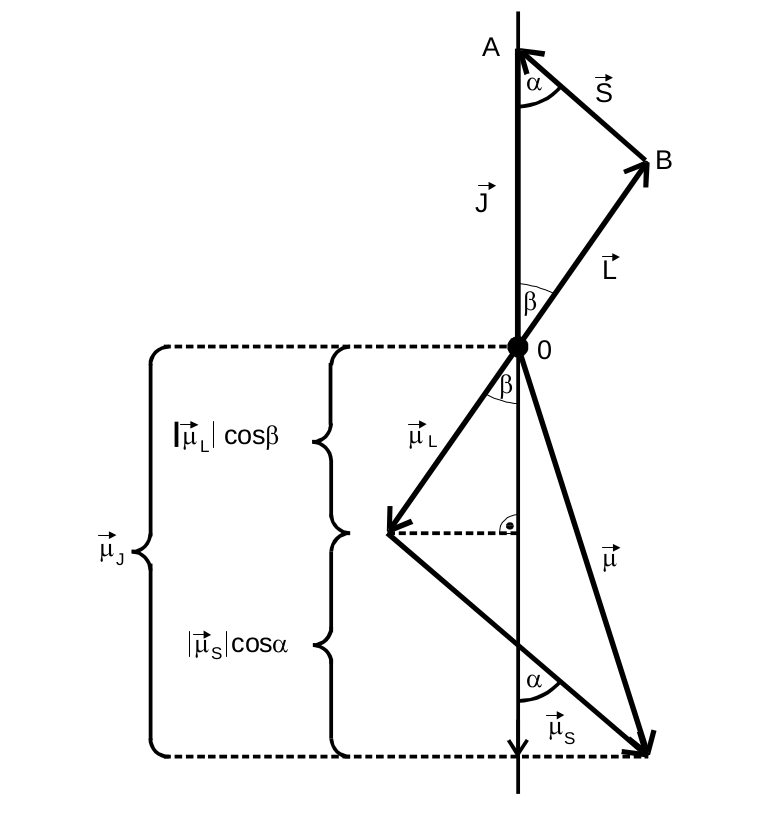
\includegraphics[width=0.55\textwidth]{../figures/vektor.png}
 \caption{Vektorielle Darstellung der magnetischen Momente und der Drehimpulse der Elektronenhülle.[Skript V606]}
 \label{fig:vektor}
\end{figure}

Mit einigen Umformungen und der Näherung aus der Quantenmechanik, dass $g_S \approx 2$ ist, vereinfacht sich Gleichung~\eqref{equ:mu_J1} zu
\begin{align}
  \label{equ:mu_J2}
  | \vec \mu_J | \approx \mu_B \sqrt{J(J+1)} \cdot \underbrace{\frac{3J(J+1) + (S(S+1)-L(L+1))}{2 J(J+1)}}_{g_J} \;
\end{align}
mit dem \emph{Landé-Faktor}
\begin{align}
  \label{equ:lande}
  g_J := \frac{3J(J+1) + (S(S+1)-L(L+1))}{2 J(J+1)} \; .
\end{align}

Ein weiteres Phänomen, das für die Berechnung von $\chi$ zu berücksichtigen ist, ist die \emph{Richtungsquantelung}. Sie folgt auch aus der Quantenmechanik und ihre Konsequenz ist, dass nur Winkel von $\vec\mu_J$ möglich sind, bei denen die z-Komponente $\mu_{J_z}$ in Richtung des externen Magnetfeldes ein ganzzahliges Vielfaches von $\mu_B g_J$ ist. Folglich gilt
\begin{align}
  \label{equ:quantelung}
  \mu_{J_z} = -\mu_B g_J m
\end{align}
mit der \emph{Orientierungsquantenzahl} $m$. Da der Betrag eines Vektors die Größe der einzelnen Komponenten beschränkt, gilt mit Gleichung~\eqref{equ:mu_J2}, dass
\begin{align*}
  |m| \leq J
\end{align*}
sein muss und damit genau $2J+1$ Einstellmöglichkeiten für den Winkel existieren. Nun ist es auch möglich ein Energieniveau in $2J+1$ Unterenergieniveaus aufzuspalten
\begin{align}
  \label{equ:Zeemann}
  E_m = -\vec \mu_J \cdot \vec B = \mu_{J_z}\cdot B = \mu_B g_J m \cdot B \; ,
\end{align}
was als \emph{Zeeman-Effekt} bezeichnet wird.
Die Magnetisierung $\vec M$ einer Substanz kann nun mit Hilfe dieser Unterenergieniveaus berechnet werden. Die Boltzmann-Verteilung gibt die Besetzungshäufigkeit $Z(E,T)$ eines Energieniveaus mit einer bestimmten Energie $E$ bei einer Temperatur $T$ an. Wird nun Gleichung~\eqref{equ:quantelung} über alle möglichen $m$ mit der zugehörigen Besetzungshäufigkeit summiert und durch die Gesamthäufigkeit aller möglichen Orientierungen geteilt, ergibt sich das gemittelte magnetische Moment. Der Betrag von $\vec M$ ist mit dem gemittelten magnetischen Moment über
\begin{align}
  M = \mu_0 N \bar \mu
\end{align}
verknüpft. Nach einigen Umformungen und Näherungen ergibt sich für die Suszeptibilität $\chi$:
\begin{align}
  \label{equ:sub_calc}
  \chi = \frac{\mu_0 \mu_B^2 g_J^2 N J(J+1)}{3k_B T} \; ,
\end{align}
mit $N$ als Anzahl der pro Volumeneinheit vorkommenden Momente, $k_B$ der Boltzmannkonstante und der Temperatur $T$. Es ist sofort zu erkennen, dass
\begin{align}
  \chi \propto \frac{1}{T}
\end{align}
ist, was als \emph{Curiesches Gesetz} des Paramagnetismus bekannt ist.\newpage

Der Paramagnetismus äußert sich besonders stark in den Atomen Seltener-Erden, da ihre Elektronenhüllen einen großen Drehimpuls aufweisen. Dies liegt an den 4f-Elektronen. Der Drehimpuls der anderen Elektronen ist abgesättigt und trägt daher nicht zum Gesamtdrehimpuls bei. Die Anordnung der Elektronen innerhalb der nicht gesättigten 4f-Schale wird durch die \emph{Hundschen Regeln} beschrieben:
\begin{itemize}
  \item Das Pauli-Prinzip bestimmt, wie sich die Einzelspins $\vec s_i$ zu dem maximalen Gesamtspin $\vec S = \sum{\vec s_i}$ kombinieren können.
  \item Der Gesamtbahndrehimpuls $\vec L = \sum{\vec l_i}$ ist die maximale Summe aus den Einzeldrehimpulsen $\vec l_i$, die weder das Pauli-Prinzip, noch die erste Regel verletzt.
  \item Wenn die Schale weniger als halb besetzt ist, ergibt sich für den Gesamtdrehimpuls $\vec J = \vec L - \vec S$, für eine mehr als die Hälfte gefüllte Schale hingegen $\vec J = \vec L + \vec S$.
\end{itemize}

\subsection{Messverfahren zur Bestimmung der magnetischen Suszeptibilität}\label{sec:messung}

Mit Hilfe einer Brückenschaltung ist es möglich die Suszeptibilität $\chi$ eines Stoffes zu messen. In Abbildung~\ref{fig:bruecke} ist eine geeignete Schaltung zu sehen.

\begin{figure}[H]
 \centering
 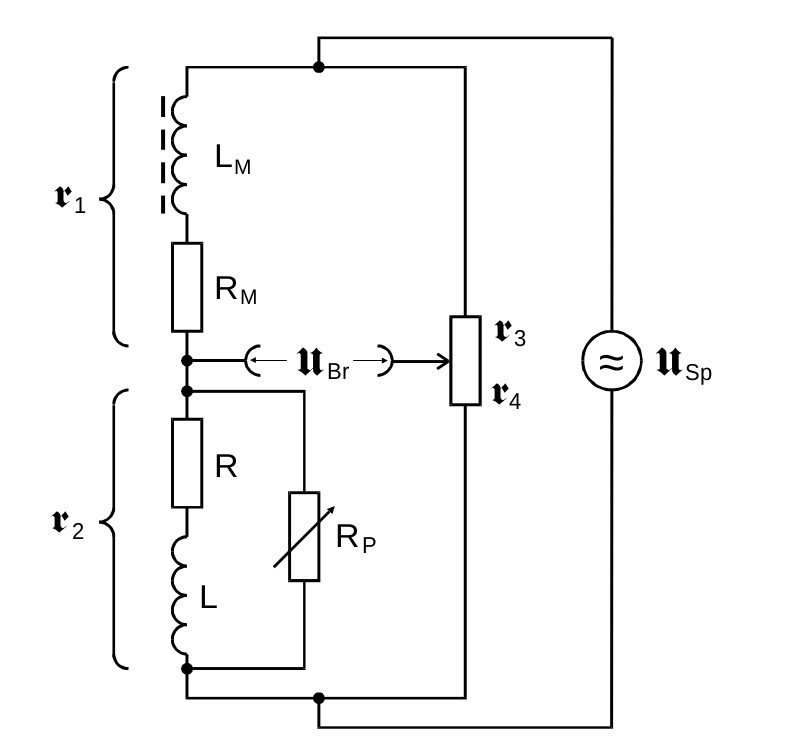
\includegraphics[width=0.55\textwidth]{../figures/bruecke.png}
 \caption{Brückenschaltung zur Messung der magnetischen Suszeptibilität.[Skript V606]}
 \label{fig:bruecke}
\end{figure}

Es werden zwei Spulen mit gleicher Induktivität benötigt, damit -- wenn eine der Spulen mit der auszumessenden Materie gefüllt wird -- die Induktivitätsdifferenz $\Delta L$ bestimmt werden kann. Da diese Differenz in der Praxis meist sehr gering ist, werden zwei möglichst identische Spulen benötigt, um eine hohe Auflösung für die Messung zu erreichen.

Es existieren zwei Methoden mit der in Abbildung~\ref{fig:bruecke} gezeigten Schaltung die Suszeptibilität zu bestimmen.
Zuerst wird die Brückenschaltung ohne Materie in den Spulen abgeglichen, d.h. die gemessene Brückenspannung $U_{\mathrm{Br}}$ wird durch die Widerstände auf den kleinst möglichen Wert eingestellt (theoretisch sollte keine Spannung mehr messbar sein).
Danach wird die Probe mit dem zu untersuchenden Material in einer der Spulen platziert und die neue Spannung gemessen. Bei hinreichend großen Frequenzen ($\omega^2 L^2 \ll R^2$) berechnet sich die Suszeptibilität nach
\begin{align}
  \label{equ:chi1}
  \chi(\omega \rightarrow \infty) = 4 \frac{F}{Q}\frac{U_{\mathrm{Br}}}{U_{\mathrm{Sp}}}
\end{align}
mit dem Querschnitt der Probe $Q$ dem Spulenquerschnitt $F$ und der Speisespannung $U_{\mathrm{Sp}}$.
Die zweite Methode besteht darin, dass nach dem einbringen der Probe nicht die Spannung gemessen, sondern der Widerstand am Potentiometer $R_3$ solange geändert wird, bis die Brückenschaltung erneut abgeglichen ist. Mit der Änderung des Widerstandes $\Delta R$ lässt sich nun die Suszeptibilität über
\begin{align}
  \label{equ:chi2}
  \chi = 2 \frac{\Delta R}{R_3}\frac{F}{Q}
\end{align}
berechnen.

\subsection{Unterdrückung von Störspannungen bei kleinen Signalspannungen}\label{sec:stoerung}
Bei Brückenschaltungen treten an den Ausgangsklemmen Störspannungen auf. Da die Brückenspannung sehr gering ist, können die Störspannungen diese nahezu vollkommen überdecken. Bei der hier vorliegenden monofrequenten Signalspannung kann dieses Problem folgendermaßen gelöst werden: Es wird ein Selektivverstärker benötigt, der wie ein elektronischer Filter wirkt und damit im Idealfall nur die monofrequente Signalspannung hindurchlässt. Die Wirksamkeit der Filterung hängt von der Güte $Q$ des Verstärkers ab: die Filterkurve (siehe Abb.~\ref{fig:glocke}) ist eine Glockenkurve deren Breite von der Güte beschrieben wird. Umso schmaler die Glockenkurve, desto besser die Unterdrückung der Störspannung. Daher ist auch klar, dass nicht alle Störspannungen vollkommen unterdrückt werden können. Des weiteren hat der Selektivverstärker den praktischen nutzen, dass er die geringe Brückenspannung verstärkt und sie somit leichter zu messen ist.

\begin{figure}[H]
 \centering
 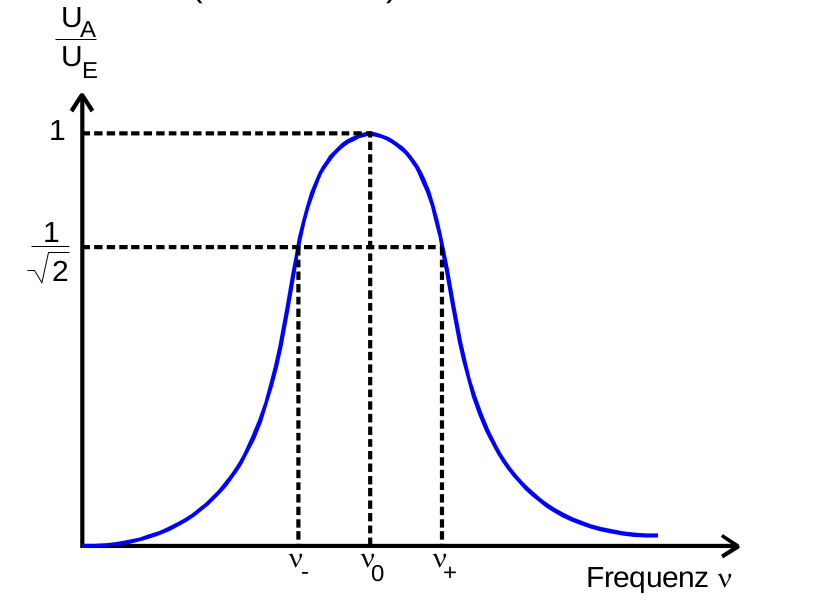
\includegraphics[width=0.4\textwidth]{../figures/glocke.png}
 \caption{Filterkurve eines Selektivverstärkers.[Skript V606]}
 \label{fig:glocke}
\end{figure}


%the end


\newpage

\section{Gaußsche Fehlerrechnung}\label{gausssche-fehlerrechnung}

\subsection{Berechnung der
Standardabweichung}\label{berechnung-der-standardabweichung}

Alle Messwerte sind als empirische Mittelwerte mit ihrer geschätzten
Standardabweichung des Mittelwertes angegeben. Diese unterschätzt die
wahre Standardabweichung, da die Wurzel aus der geschätzten Varianz
gezogen wird. Der arithmetische Mittelwert ist definiert als

\begin{align}
    \bar x = \frac{1}{n} \  \sum_{i=1}^n x_i \  .
    \label{equ:mean}
\end{align}

Die geschätzte Standardabweichung ist gegeben durch

\begin{align}
    s = \sqrt{\frac{1}{n-1} \sum_{i=1}^n (x_i - \bar x)^2}
    \label{equ:s}
\end{align}

mit der geschätzten Standardabweichung des Mittelwertes als

\begin{align}
    \Delta \bar x = \frac{s}{ \sqrt{n} }
    \label{equ:stdofmean}
\end{align}

\subsection{Gaußsche
Fehlerfortpflanzung}\label{gausssche-fehlerfortpflanzung}

Das Berechnen von Funktionen mit fehlerbehafteten Parametern erfolgt
mittels der Gauß'schen Fehlerfortpflanzung

\begin{align}
    \Delta f = \sqrt{ \sum_{i=1}^n \left( \frac{\diff f}{\diff y_i} \right)^2 (\Delta y_i)^2} \qquad \qquad \mathrm{mit} \quad f(y_1, \ldots , y_n)
    \label{equ:gauss}
\end{align}

\newpage
\section{Aufbau und Durchführung}\label{sec:aufbau-und-durchfuehrung}
Wie in Abschnitt~\ref{sec:messung} beschrieben, wird zur Messung der Suszeptibilität eine Brückenschaltung wie in Abbildung~\ref{fig:bruecke} benötigt. Um die in Abschnitt~\ref{sec:stoerung} erläuterten Störspannungen zu unterdrücken und die Brückenspannung messen zu können, wird die in Abbildung~\ref{fig:schaltung} gezeigte Schaltung verwendet.

\begin{figure}[H]
 \centering
 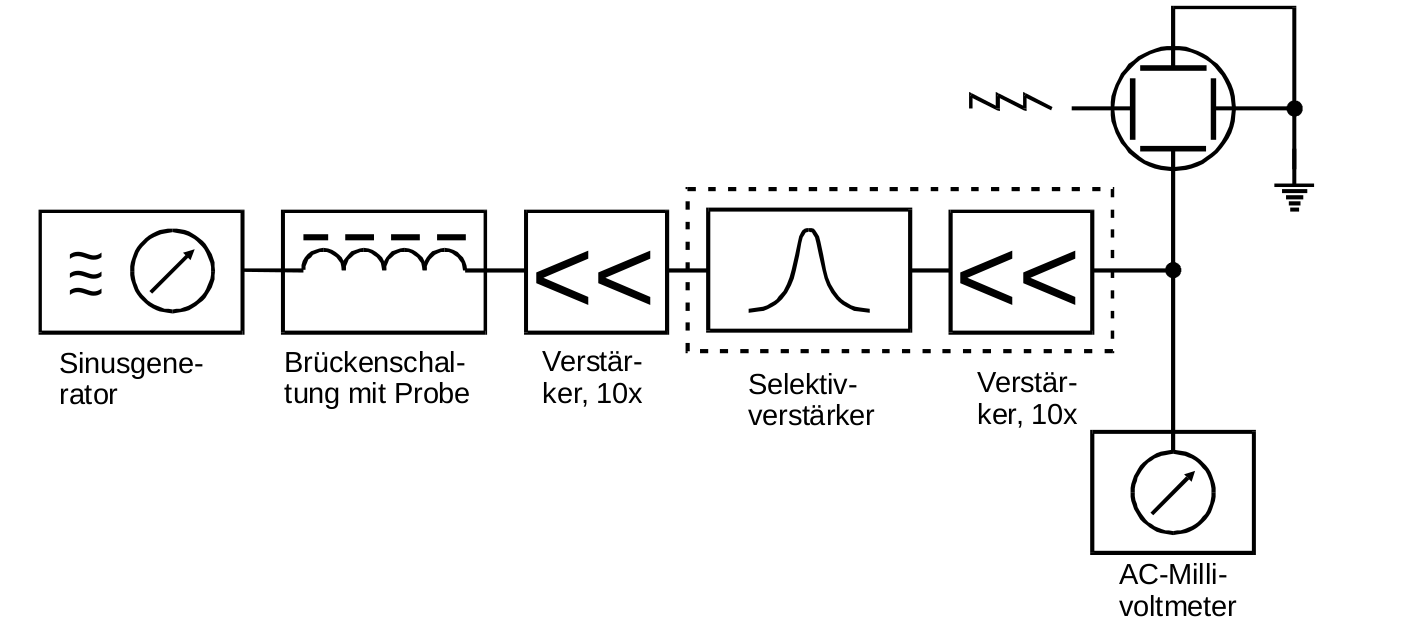
\includegraphics[width=1\textwidth]{../figures/schaltung.png}
 \caption{Schaltbild der zur Messung der Suszeptibilität verwendeten Apparatur.[Skript V606]}
 \label{fig:schaltung}
\end{figure}

Zunächst wird nur der Selektivverstärker bei einer Güte von $Q = 100$ untersucht. Mit Hilfe eines Sinusgenerators wird bei konstanter Eingangsspannung $U_E$ die Ausgangsspannung $U_A$ (am Verstärker) in einem Bereich von 30~-~40~$\si{\kilo\hertz}$ ausgemessen. So lässt sich die Filterkurve des Selektivverstärkers erstellen. Dabei sollte im Bereich der Durchlassfrequenz genauer, also etwa in $\SI{0.1}{\kilo\hertz}$-Schritten, gemessen werden. Aus der Filterkurve kann dann die Durchlassfrequenz ermittelt werden, bei der die Ausgangsspannung maximal wird. Bei dieser Frequenz wird die Messung zur Suszeptibilität durchgeführt, da dort die Störspannungen am besten herausgefiltert werden und die Brückenspannung am genauesten gemessen werden kann.

Nun wird die in Abbildung~\ref{fig:schaltung} dargestellte Schaltung aufgebaut und die Signalfrequenz auf die Durchlassfrequenz des Selektivverstärkers eingestellt, außerdem wird die Speisespannung $U_{Sp}$ notiert.
Mit Hilfe der ersten Methode aus Abschnitt~\ref{sec:messung} wird die Brückenschaltung abgeglichen und die Einstellung des $R_3/R_4$ Widerstandes sowie die -- aufgrund der Störspannungen trotzdem noch -- zu messende Brückenspannung $U_{Br}$ abgelesen. Die Länge der Probe wird ausgemessen, ihre Masse kann einfach abgelesen werden. Daraufhin wird die Probe in einer der Spulen platziert und die Änderung der Brückenspannung wird notiert. Als nächstes wird direkt mit der zweiten Methode weiter gemessen, indem der Widerstand $R_3/R_4$ solange variiert wird, bis die Brückenspannung wieder minimal ist. Auch diese Widerstands-Einstellung wird aufgeschrieben. Die Messung wird für jedes Material dreimal wiederholt. Insgesamt werden drei verschiedene Seltene-Erd-Verbindungen gemessen.

%Der Aufbau ist in Abbildung~\ref{fig:aufbau} zu sehen.
%\begin{figure}[H]
% \centering
% \includegraphics[width=\textwidth]{../figures/aufbau.png}
% \caption{Versuchsapparatur. [Skript V602]}
% \label{fig:aufbau}
%\end{figure}

\section{Auswertung}
\label{sec:Auswertung}

	\subsection{Filterkurve}
	\label{sub:Filterkurve}
		\begin{figure}[H]
			\centering
			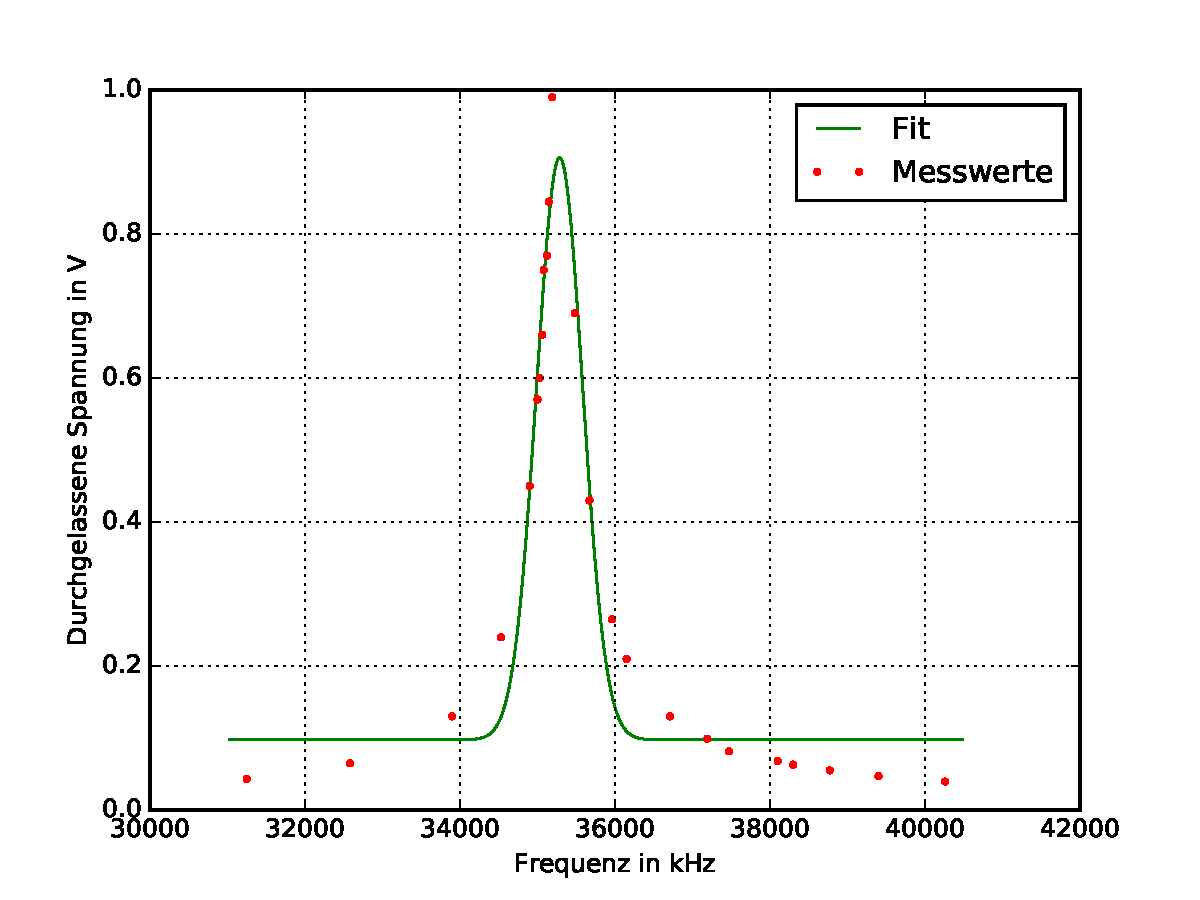
\includegraphics[width=\textwidth]{../plots/amplifier.pdf}
			\caption{Durchlasskurve des Selektiv-Verstärkers. Der Fit der Gaußkurve dient nur zum finden der Bandbreite; es reicht deswegen aus, dass dieser nur in der Nähe von $U = \nicefrac{1}{\sqrt{2}}\si{\V}$ genau ist.}
			\label{fig:_plots_amplifier_pdf_}
		\end{figure}

		Bei einer theoretischen Güte von 100 ist der Bandpass des Filters recht scharf. Die aus den Messdaten gewonnene Kurve hat eine Güte von

		\begin{align}\label{equ:guete}
			Q=\nicefrac{f_\text{Umax}}{f_\text{Bandbreite}} = 77.16 \;.
		\end{align}

		Das Spannungsmaximum von \SI{0.99}{\V} bei einer Speisespannung von etwa \SI{1}{\V} wird bei etwa \SI{35.19}{\k\Hz} eingenommen. Die Speisespannung bleibt in den folgenden Abschnitten gleich.
		Die Kurve wird ohne Verstärkung der Spannung aufgenommen.

	\subsection{Suszeptibilität}
	\label{sub:suszeptibilität}
		
		Die Suszeptibilität wird durch das Messen der Brückenspannung nach Stabeinführung ($\chi_U$) und das Vergleichen der Widerstände bei abgeglichener Brücke ($\chi_R$) bestimmt. Diese Werte weichen stark voneinander ab, der Mittelwert aus beiden liegt jedoch recht nahe an dem nach der Hund'schen Regel berechneten $\chi_\text{Hund}$.  
		Die Messungen werden mit einer um den Faktor 100 verstärkten Spannung durchgeführt.

		Die mithilfe der Hund'sche Regel bestimmten Parameter sind in Tabelle~\ref{tab:elektronenkonf} zu sehen; aus ihnen ergibt sich mit Gl.~\ref{equ:sub_calc} die Werte aus Tabelle~\ref{tab:results}. Es werden 15°C als Raumtemperatur angenommen.

		Zur besseren Einschätzung der Werte dient Abbildung~\ref{fig:_plots_chi_pdf}.

		\begin{table}[H]
		    \centering
		    \caption{Elektronenkonfiguration der 4f-Schale.}
		    \label{tab:elektronenkonf}
		    \begin{adjustbox}{center}
		    \begin{tabular}{
		        r
		        S
		        S
		        S}
		     \toprule
		     \multicolumn{1}{c}{} &
		     \multicolumn{1}{c}{$\text{Dy}^{3+}$} &
		     \multicolumn{1}{c}{$\text{Nd}^{3+}$} &
		     \multicolumn{1}{c}{$\text{Gd}^{3+}$} \\
		     \midrule
		     \primitiveinput{../tables/hund_params.tex}
		     \bottomrule
		    \end{tabular}
		    \end{adjustbox}
		\end{table}

		\begin{table}[H]
		    \centering
		    \caption{Messergebnisse beider Methoden und Vergleich mit der Hund'schen Regel. Die letzte Spalte bezeichnet die relative Abweichungen der verschiedenen Werte von den Vorhersagen nach Hund.}
		    \label{tab:results}
		    \begin{adjustbox}{center}
		    \begin{tabular}{
		    	r
		        r@{$\pm$}l
		        r@{$\pm$}l
		        c
		        c
		        c
		        c
		        c}
		     \toprule
		     \multicolumn{1}{c}{}&
		     \multicolumn{6}{c}{Suszeptibilitäten}&
		     \multicolumn{3}{c}{Abweichungen in \%}\\
		     \multicolumn{1}{c}{Ion} &
		     \multicolumn{2}{c}{$\chi_U$} &
		     \multicolumn{2}{c}{$\chi_R$} &
		     \multicolumn{1}{c}{$\chi_\text{mittel}$}&
		     \multicolumn{1}{c}{$\chi_\text{Hund}$}&
		     \multicolumn{1}{c}{$\chi_U$}&
		     \multicolumn{1}{c}{$\chi_R$}&
		     \multicolumn{1}{c}{$\chi_\text{mittel}$}\\
		     \midrule
		     \primitiveinput{../tables/chi-results.tex}
		     \bottomrule
		    \end{tabular}
		    \end{adjustbox}
		\end{table}

		\begin{figure}[H]
			\centering
			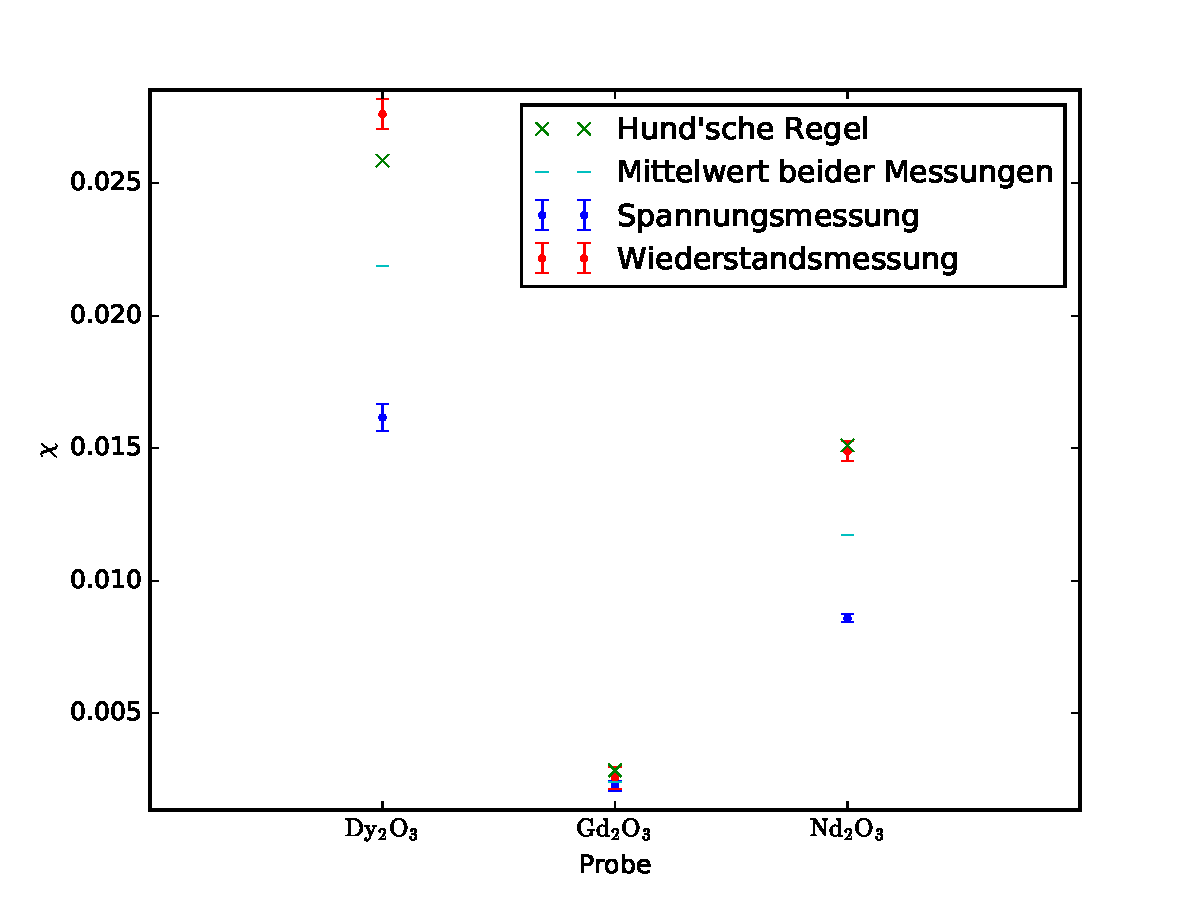
\includegraphics[width=\textwidth]{../plots/chi.pdf}
			\caption{Suszeptibilität der Proben im Vergleich.}
			\label{fig:_plots_chi_pdf}
		\end{figure}



	\subsection{Messdaten}
	\label{sub:messdaten}
		Da die Proben aus einem Pulver bestehen ist ihre Dichte geringer als die Dichte eines Einkristalls $\rho$. Mit der Masse $m$ der Probe und ihrer Länge $L$
		lässt sich der effektive Querschnitt $Q_\text{adj}$ berechnen:

			\begin{align*}
				Q_\text{adj} = \frac{m}{L \rho} \;.
			\end{align*}

		Die benutzte Spule hat einen Durchmesser von \SI{86.6}{10^{-6}\m^2}, die Brückenschaltung hat einen Nebenwiderstand von $R_3=\SI{998}{\ohm}$.
		Es folgt eine Auflistung der Messdaten und der daraus berechneten Zwischenergebnisse.

		\begin{table}[H]
		    \centering
		    \caption{Parameter der Proben.}
		    \label{tab:seern}
		    \begin{adjustbox}{center}
		    \begin{tabular}{
		    	l
		        S
		        S
		        S}
		     \toprule
		     \multicolumn{1}{c}{} &
		     \multicolumn{1}{c}{$\text{Dy}_2 \text{O}_3$} &
		     \multicolumn{1}{c}{$\text{Nd}_2 \text{O}_3$} &
		     \multicolumn{1}{c}{$\text{Gd}_2 \text{O}_3$} \\
		     \midrule
		     \primitiveinput{../tables/proben_parameter.tex}
		     \bottomrule
		    \end{tabular}
		    \end{adjustbox}
		\end{table}

		\begin{table}[H]
		    \centering
		    \caption{Messdaten zu Dy.}
		    \label{tab:mess_dy}
		    \begin{adjustbox}{center}
		    \begin{tabular}{
		        c
		        c
		        c
		        c}
		     \toprule
		     \multicolumn{1}{c}{$\chi_U$} &
		     \multicolumn{1}{c}{$U$ in \si{\nano \V}} &
		     \multicolumn{1}{c}{$\chi_R$} &
		     \multicolumn{1}{c}{$\Delta R$ in \si{\ohm}} \\
		     \midrule
		     \primitiveinput{../tables/data_element_0.tex}
		     \bottomrule
		    \end{tabular}
		    \end{adjustbox}
		\end{table}

		\begin{table}[H]
		    \centering
		    \caption{Messdaten zu Nd.}
		    \label{tab:mess_dy}
		    \begin{adjustbox}{center}
		    \begin{tabular}{
		        c
		        c
		        c
		        c}
		     \toprule
		     \multicolumn{1}{c}{$\chi_U$} &
		     \multicolumn{1}{c}{$U$ in \si{\nano \V}} &
		     \multicolumn{1}{c}{$\chi_R$} &
		     \multicolumn{1}{c}{$\Delta R$ in \si{\ohm}} \\
		     \midrule
		     \primitiveinput{../tables/data_element_1.tex}
		     \bottomrule
		    \end{tabular}
		    \end{adjustbox}
		\end{table}

		\begin{table}[H]
		    \centering
		    \caption{Messdaten zu Gd.}
		    \label{tab:mess_dy}
		    \begin{adjustbox}{center}
		    \begin{tabular}{
		        c
		        c
		        c
		        c}
		     \toprule
		     \multicolumn{1}{c}{$\chi_U$} &
		     \multicolumn{1}{c}{$U$ in \si{\nano \V}} &
		     \multicolumn{1}{c}{$\chi_R$} &
		     \multicolumn{1}{c}{$\Delta R$ in \si{\ohm}} \\
		     \midrule
		     \primitiveinput{../tables/data_element_2.tex}
		     \bottomrule
		    \end{tabular}
		    \end{adjustbox}
		\end{table}
\section{Diskussion}
\label{sec:Diskussion}

Die Durchlasskurve des Bandpasses scheint ausreichend scharf zu sein, um Störungen zuverlässig zu beseitigen. Die Spannungsmesswerte
zeigen nur eine kleine Streuung auf (vergl. $\chi$-Fehler in Tabelle~\ref{tab:results}).

Die Unterschiede zwischen den beiden Messmethoden sind jedoch gravierend: Während die durch Abgleichen der Brücke gewonnenen Messwerte gut zu den Vorhersagen der Theorie passen, weichen die Spannungsmesswerte sehr stark ab. Dies liegt vermutlich an der Spannungsquelle: Diese musste nach dem Vermessen der Güte gewechselt werden. Die Frequenz ließ sich an der zweiten Quelle nur grob einstellen, sodass wahrscheinlich eine Frequenz gewählt wurde, die nicht mehr in der Nähe des Peaks der Durchlasskurve liegt.
%und so maximal deutlich weniger als die \SI{1}{\volt} der Speisespannung gemessen werden kann.
Dies würde alle Messwerte der Spannungsmessmethode stark verfälschen, die durch abgleichen der Brücke gewonnene Messwerte jedoch unberührt lassen.

Während der Messung war zu bemerken, dass ein Drehen der Probe in der Spule eine dauerhafte Spannungsänderung in der Brücke
bewirkte. Die Proben waren scheinbar nicht isotrop.

Eine weitere Fehlerquelle liegt in der Abschätzung des Probendurchmessers. Die Länge des in der Spule befindlichen Teils
der Probe ist von außen nicht klar zu beurteilen.

\newpage
\section{Literaturangabe}
\label{sec:Literatur}

Bilder und Daten aus dem Skript zu \emph{Messung der Suszeptibilität paramagnetischer Substanzen}, Versuch 606, TU Dortmund, abrufbar auf:\\
\url{http://129.217.224.2/HOMEPAGE/PHYSIKER/BACHELOR/AP/SKRIPT/V606.pdf}\\(Stand 30.05.16)\par


NIST, \emph{Theoriewerte der physikalischen Konstanten}, abrufbar auf:\\
\url{http://physics.nist.gov/cuu/index.html}\\
(Stand 16.05.16)\par

% NIST, \emph{Elektronen Masse}, abrufbar auf:\\
% \url{http://physics.nist.gov/cgi-bin/cuu/Value?me}
% (Stand 16.05.16)\par

% NIST, \emph{Plancksches Wirkungsquantum}, abrufbar auf:\\
% \url{http://physics.nist.gov/cgi-bin/cuu/Value?h|search_for=planck}
% (Stand 16.05.16)\par

% NIST, \emph{Boltzmannkonstante}, abrufbar auf:\\
% \url{http://physics.nist.gov/cgi-bin/cuu/Value?k|search_for=boltzmann}
% (Stand 16.05.16)\par


%\printbibliography
%\end{multicols}
\end{document}
